Предложенный в предыдущей дипломной работе подход предназначен для решения задач анализа строковых данных, обладающих некоторого рода синтаксической структурой, которая, наряду с непосредственно символами рассматриваемых строк, является важным источником информации о каких-либо характеристиках входных данных, но при этом оказывается слишком сложной для формализации.

В рамках данного подхода характерные элементы синтаксической структуры необходимо описать средствами формальной грамматики, а для поиска во входных данных подстрок, подходящих под это описание, использовать алгоритм синтаксического анализа. Затем извлеченные парсером элементы синтаксической структуры предлагается использовать в процессе обучения нейронных сетей, спроектированных для решения поставленной задачи. Основная идея такого комбинирования формальных грамматик и нейронных сетей заключается в том, что достаточно простая грамматика призвана формализовать только базовые и, вероятно, неполные законы образования синтаксической структуры последовательностей, и предполагается, что нейронной сети будет достаточно этой информации для выявления уже более комплексных, стохастических закономерностей, необходимых для решения некоторой аналитической задачи. Стоит отметить, что в первоначальной формулировке данный подход не ограничивает ни спектр решаемых задач, ни используемые типы грамматик и технологии, а лишь описывает набор действий для обработки определенного класса данных. Соответствующая архитектура с точки зрения физической реализации представлена на рис.~\ref{diagram}, и необходимыми компонентами для проведения любого рода экспериментальных исследований в рамках предлагаемого подхода являются модули для синтаксического анализа и нейронных сетей, хранилище всех необходимых данных (входных последовательностей, метаданных и т.д.), а также --- формальная грамматика, представленная в принимаемом парсером формате.

\vspace{5mm}
\begin{figure}[h]
\begin{center}
\centering
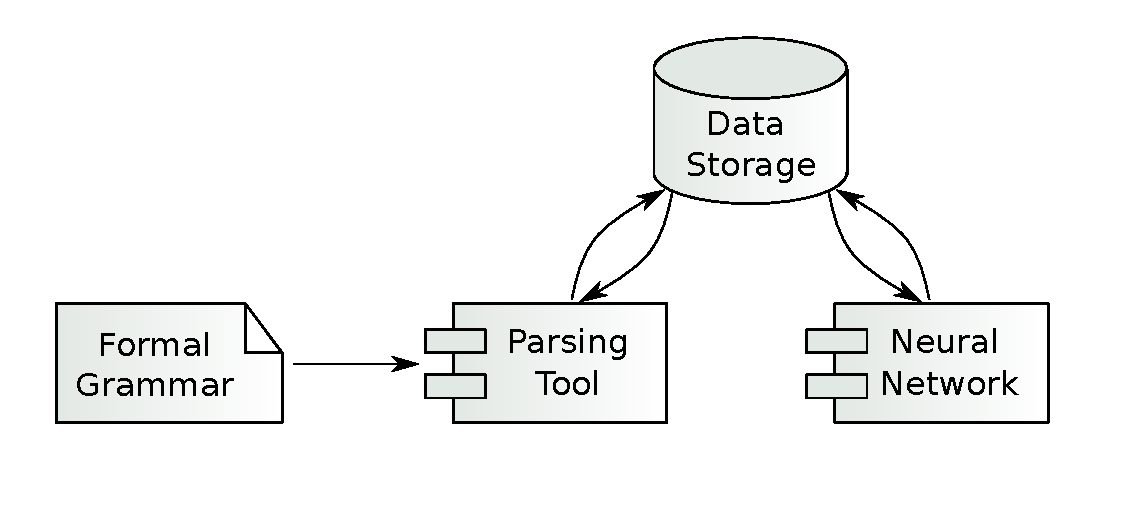
\includegraphics[width=12.0cm]{pics/diagram.pdf}
\caption{Архитектурные компоненты предложенного подхода}
\label{diagram}
\end{center}
\end{figure} 

Одной из потенциальных областей применения такого подхода является биоинформатика, в частности, различные задачи анализа РНК, где в качестве символьных последовательностей можно рассмотреть нуклеотидные цепочки РНК различных организмов, а в качестве синтаксической структуры --- биологическую вторичную структуру молекулы РНК. В текущей работе исследуется возможность применения описанного выше подхода для решения задачи предсказания вторичной структуры РНК. Далее будет описана разработанная для этого архитектура решения, включающая в себя два основных шага: задание грамматики для поиска характерных элементов вторичной структуры, а затем -- проектирование и обучение нейронных сетей, генерирующих для последовательности РНК максимально близкую к реальной вторичную структуру на основе полученных с помощью парсера данных.

\subsection{Формальная грамматика}
Первичная структура молекулы РНК представляет собой цепочку из нуклеотидов четырех типов (аденин, цитозин, гуанин и урацил), что в терминах синтаксического анализа есть последовательность символов алфавита \{A, C, G, U\}; вторичная же структура образовывается вследствие того, что некоторые участки первичной соединяются между собой, формируя рекурсивную композицию из шпилек разного размера и степени вложенности. Обобщенный вид таких шпилек может быть формализован средствами достаточно простой контекстно-свободной грамматики, каковой является используемая в данной работе грамматика $G_0$ (рис.~\ref{gram}). Грамматика учитывает только Уотсон-Криковские правила формирования нуклеотидных пар $A-U$, $C-G$ (строка \textbf{5}) и описывает рекурсивные композиции шпилек высоты от трех и более (строки \textbf{7-12}). Размер петли внутри шпильки лежит в пределах от одного до двадцати нуклеотидов, и такую же длину имеют последовательности, расположенные между любыми двумя шпильками (строка \textbf{2}). Эти числа были выбраны путем балансирования между следующими двумя соображениями: соответствие эмпирическим наблюдениям биологических данных и адекватность напрямую зависящих от длины и сложности грамматики временных затрат на работу парсера. По тем же причинам в $G_0$ не были включены неканонические нуклеотидные связи, которые могут встречаться в реальной вторичной структуре РНК --- для того, чтобы учесть все возможные пары нуклеотидов, придется ввести большое количество правил, имеющих вероятностную природу. Кроме того, средствами контекстно-свободных грамматик невыразимы псевдоузлы, однако псевдоузел есть комбинация из двух шпилек, следовательно, $G_0$, не описывая псевдоузел как единое целое, позволяет, тем не менее, выделить из входной последовательности обе составляющие его подстроки. Здесь становится понятным основное отличие нашего подхода от классического использования формальных грамматик в данной области~\cite{knudsen1999rna,dowell2004evaluation,rivas2000language} --- мы не пытаемся ни смоделировать вторичную структуру целиком, ни описать все возможные закономерности ее образования, но разбиваем ее на простые составные части, синтезировать из которых более сложные объекты предлагается уже с помощью нейронных сетей, что кратно уменьшает интеллектуальные и вычислительные затраты на синтаксический анализ.

\begin{figure}[h]
\begin{Verbatim}[numbers=left,xleftmargin=5mm]
s1: stem<s0>
any_str : any_smb*[1..20]
s0: any_str | any_str stem<s0> s0
any_smb: A | U | C | G
stem1<s>: A s U | G s C | U s A | C s G 
stem2<s>: stem1< stem1<s> >
stem<s>:  
      A stem<s> U 
    | U stem<s> A 
    | C stem<s> G 
    | G stem<s> C 
    | stem1< stem2<s> >  
\end{Verbatim}
\caption{Контекстно-свободная грамматика $G_0$ для описания шпилек вторичной структуры РНК}
\label{gram}
\end{figure}

Рассмотрим теперь формальный вид и практический смысл результата работы синтаксического анализатора для вышеописанной грамматики и последовательности РНК некоторого организма. Синтаксический анализ в данном случае используется для поиска всех подстрок входной строки, выводимых из стартового нетерминала $s1$ грамматики $G_0$, иными словами, для поиска тех участков этой строки, которые, в терминах $G_0$, могут свернуться в шпильки при формировании вторичной структуры. Формально, для входной строки $w$ парсер заполнит верхнетреугольную булеву матрицу --- матрицу разбора $M_P$, где $M_P[i,j]=1 \iff$ подстрока $w[i..j]$ выводится в $G_0$. Так как интересующие нас шпильки должны иметь высоту от трех, каждой шпильке высоты $n$ в матрице разбора будет соответствовать цепочка из $n - 2$ единиц. На рис.~\ref{mtrx} представлен результат работы парсера для изображенного на рис.~\ref{rna_a} случая последовательности, сворачивающейся в шпильку высоты четыре. Каждой нуклеотидной связи, образующей шпильку высоты от трех (сплошные линии голубого цвета), соответствует единица в ячейке матрицы разбора, при этом очевидно, что шпилька высоты три инкапсулирует в себе шпильки высоты два и один, обозначенные на рисунке пунктирными линиями. Помимо уже знакомой нам шпильки с рис.~\ref{rna_a}, в данной строке парсер обнаружил еще одну выводимую в грамматике подстроку (единица в позиции $[0,11]$): таким образом, для рассматриваемой цепочки существует два теоретически возможных варианта свертки, из которых реализованным на практике оказался только один.

\begin{figure}[h]
\begin{center}
\centering
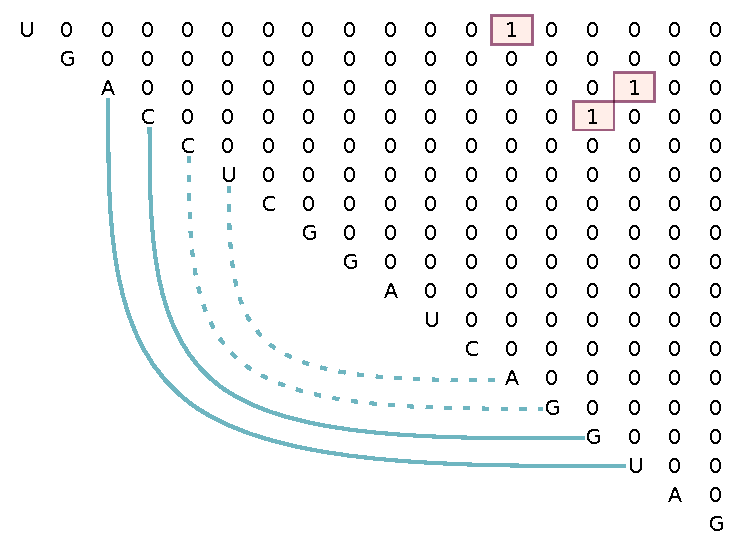
\includegraphics[width=10.0cm]{pics/matrix.pdf}
\caption{Матрица разбора для последовательности РНК}
\label{mtrx}
\end{center}
\end{figure} 
\vspace{3mm}

Остановимся в контексте предложенного подхода на проблеме обработки псевдоузлов, которые, как уже упоминалось ранее, не выводимы в используемой грамматике $G_0$. На рис.~\ref{pk_a} представлен пример последовательности, сворачивающейся в псевдоузел, а на рис.~\ref{pk_b} --- соответствующая данной последовательности матрица разбора. Рассматриваемый псевдоузел состоит из двух взаимопересекающихся шпилек высоты три и четыре, каждая из которых по отдельности выводима в $G_0$ и, следовательно, будет отражена в матрице разбора одной и двумя единицами соответственно. Несмотря на то, что на этапе синтаксического анализа еще не известно, образуют ли эти две найденные шпильки псевдоузел или же являются просто двумя теоретически возможными вариантами свертки цепочки, для нашего подхода предсказание псевдоузлов не становится ни сложностью, ни ограничением, так как матрицы разбора содержат всю необходимую о них информацию, которая должна быть более четко интерпретирована уже на этапе анализа данных нейронными сетями.

\captionsetup[subfigure]{justification=centering}
\begin{figure}[h]
\centering
\begin{subfigure}{.3\textwidth}
  \centering
  \fbox{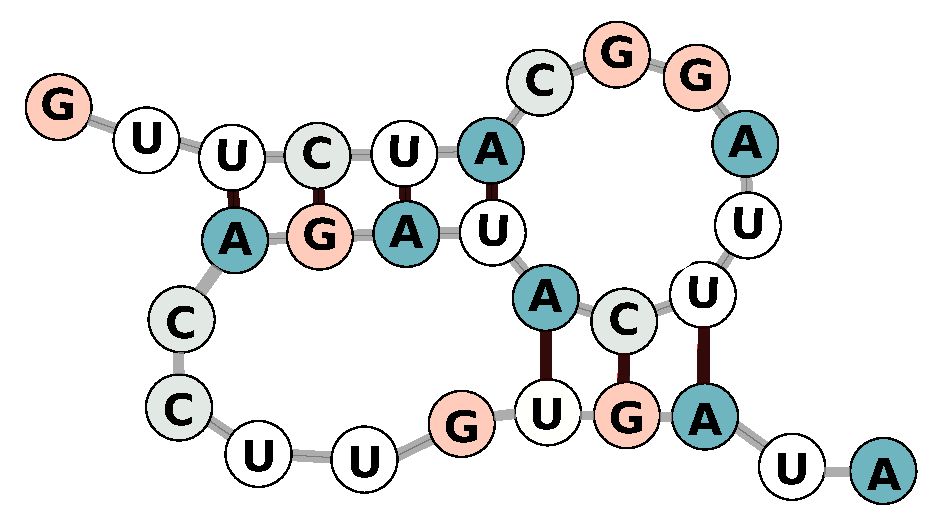
\includegraphics[width=.9\linewidth]{pics/pk.pdf}}
  \caption{Псевдоузел}
  \label{pk_a}
\end{subfigure}%
\begin{subfigure}{.7\textwidth}
  \centering
  \fbox{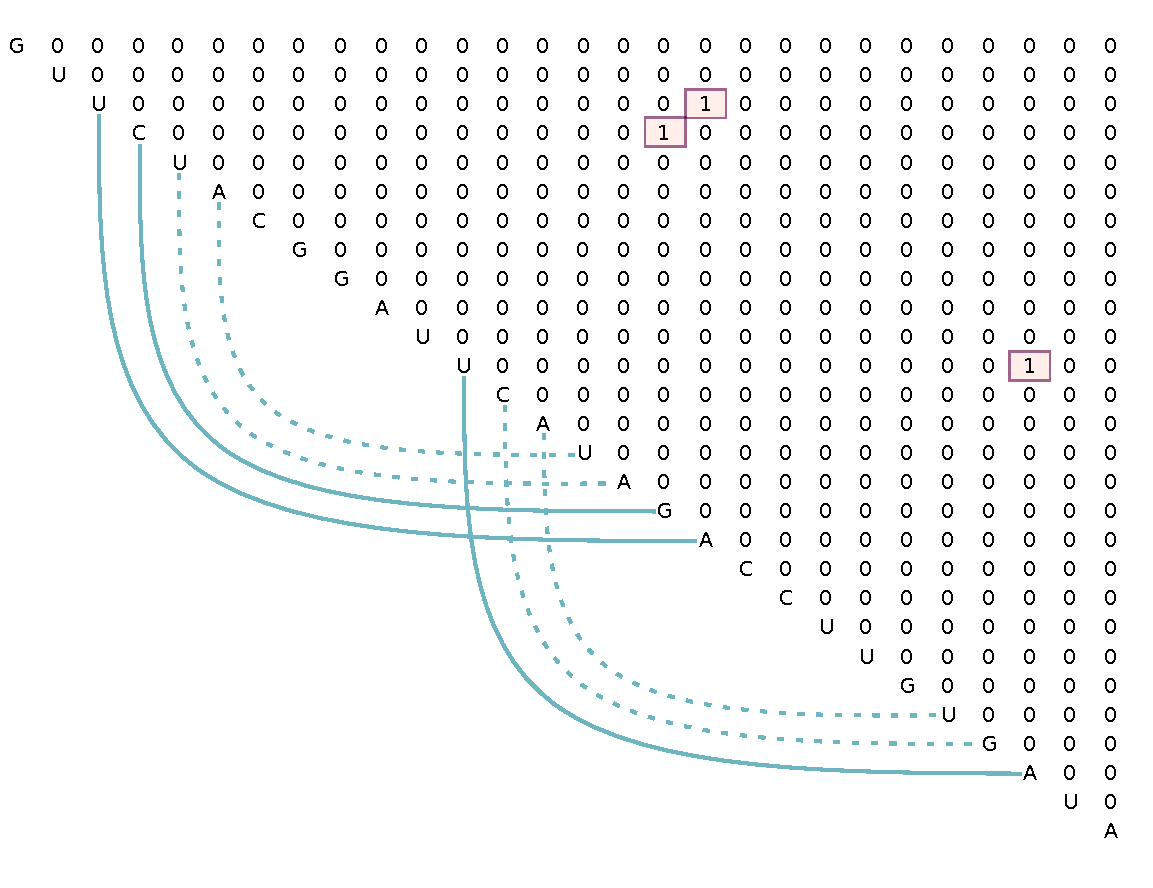
\includegraphics[width=.9\linewidth]{pics/matrix2.pdf}}
  \caption{Матрица разбора для последовательности с псевдоузлом}
  \label{pk_b}
\end{subfigure}
\caption{Обработка псевдоузлов в рамках предложенного подхода}
\label{pk}
\end{figure}

Таким образом, матрицы разбора хранят информацию о всех возможных расположениях шпилек вторичной структуры во входных последовательностях, однако на данный момент это только теоретические, искусственные объекты, для соотнесения которых с реальными биологическими данными требуется последующая обработка, и об этом будет подробно рассказано в следующем разделе.

\subsection{Нейронная сеть}
На данном этапе поставленная задача конкретизируется до следующей --- разработать нейронную сеть, которая принимает на вход матрицы, полученные синтаксическим анализатором по грамматике $G_0$ для некоторого набора последовательностей РНК, и, обучаясь на вторичных структурах, предоставленных в качестве эталонных для рассматриваемых последовательностей, оптимизирует параметры для преобразования матриц разбора в корректные вторичные структуры. Данный раздел посвящен описанию всех тонкостей этого процесса. 

\subsubsection{Подготовка данных} 
Входные данные для нейросети (матрицы разбора) были описаны в прошлом разделе, и теперь необходимо определить источник и формат эталонных данных. Существуют специализированные биологические базы данных, в которых размещены цепочки РНК различных организмов вместе с их извлеченными из природного материала или же полученными надежными методами вторичными структурами. Такие данные оптимальны для валидации, а, следовательно, и для обучения предсказывающих вторичную структуру алгоритмов. 

Как правило, в базах данных вторичные структуры РНК хранятся в скобочной (dot-bracket) нотации, из которой легко получить еще один классический формат  представления вторичной структуры --- так называемую матрицу контактов (contact map). Матрица контактов описывает наличие или отсутствие связи между каждыми двумя нуклеотидами последовательности: формально, для строки $w$ это верхнетреугольная булева матрица $M_C$, где $M_C[i,j]=1 \iff w[i]$ и $w[j]$ образуют пару во вторичной структуре. Как было описано в прошлом разделе, результат работы парсера на входной строке $w$ --- верхнетреугольная булева матрица $M_P$, где $M_P[i,j]=1 \iff w[i..j]$ свернется в шпильку по правилам грамматики. Нетрудно проверить, что наличие контакта между нуклеотидами $w[i]$ и $w[j]$ эквивалентно тому факту, что последовательность $w[i..j]$ является шпилькой, поэтому, несмотря на то, что наше определение вторичной структуры как композиции вложенных шпилек не относится к общеупотребимым, матрицу разбора можно также описать как матрицу контактов, формируемых только выразимыми в грамматике элементами. Таким образом, использование матричного представления вторичной структуры при подготовке эталонных данных для нейронной сети представляется самым удобным в свете специфики используемых в качестве входных данных матриц разбора. 

Для наглядности и удобства применения нейронных сетей мы предлагаем смотреть на матрицу контактов и матрицу разбора как на изображения: пикселями белого цвета обозначим позиции в матрицах с единицами, черного --- с нулями. Матрицы разбора содержат $n - 2$ единицы для каждой шпильки высоты $n>3$, следовательно, в качестве предобработки перед обучением нейросети для каждой единицы в матрице разбора следует добавить еще две единицы в направлении главной диагонали. Кроме того, сама нуклеотидная последовательность РНК может содержать некоторую важную информацию, поэтому предлагается закодировать ее на главной диагонали изображений равноотстающими друг от друга серыми пикселями. 

На рисунке~\ref{struc} продемонстрировано, как для одной и той же последовательности РНК будут выглядеть входной и эталонный образцы для нейронной сети, а также показана визуализация соответствующей вторичной структуры. Контакты, относящиеся к трем присутствующим в рассматриваемой цепочке шпилькам, на всех изображениях выделены голубым, сиреневым и розовым цветами. Данный рисунок является наглядным примером того, что далеко не все найденные парсером шпильки будут представлены в реальной вторичной структуре (белые пиксели изображения~\ref{struc_c}). Кроме того, видно, что в сгенерированной синтаксическим анализатором матрице отсутствует несколько эталонных контактов: в данном случае это произошло из-за того, что они были образованы непредусмотренными грамматикой неканоническими нуклеотидными парами. 

\captionsetup[subfigure]{justification=centering}
\begin{figure}[h]
\centering
\begin{subfigure}{.3\textwidth}
  \centering
  \fbox{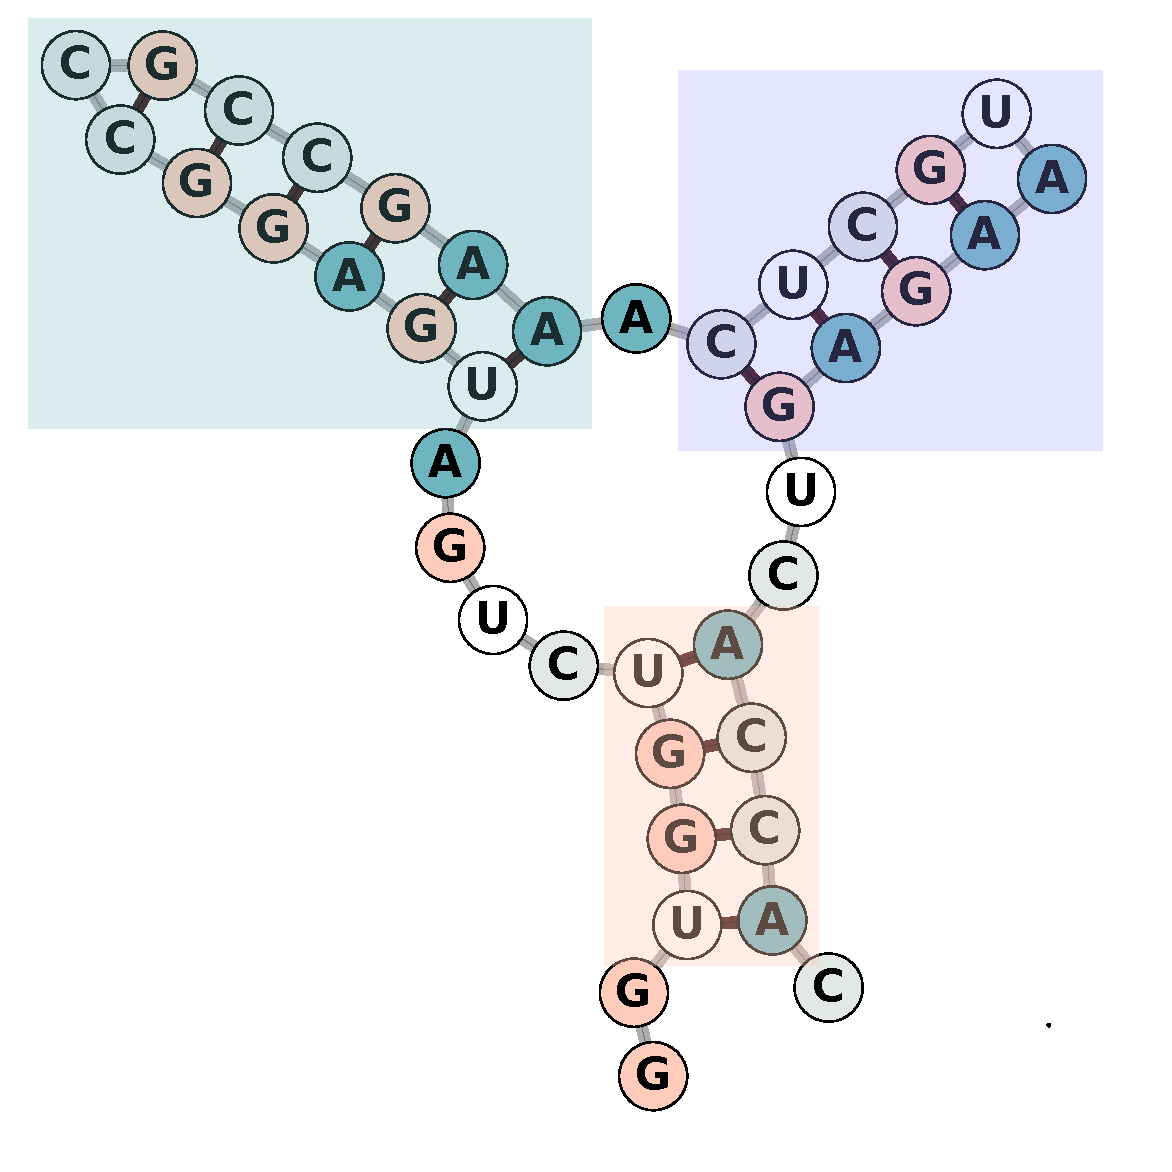
\includegraphics[width=.9\linewidth]{pics/struct.pdf}}
  \caption{Визуализация вторичной структуры}
  \label{struc_a}
\end{subfigure}%
\begin{subfigure}{.3\textwidth}
  \centering
  \fbox{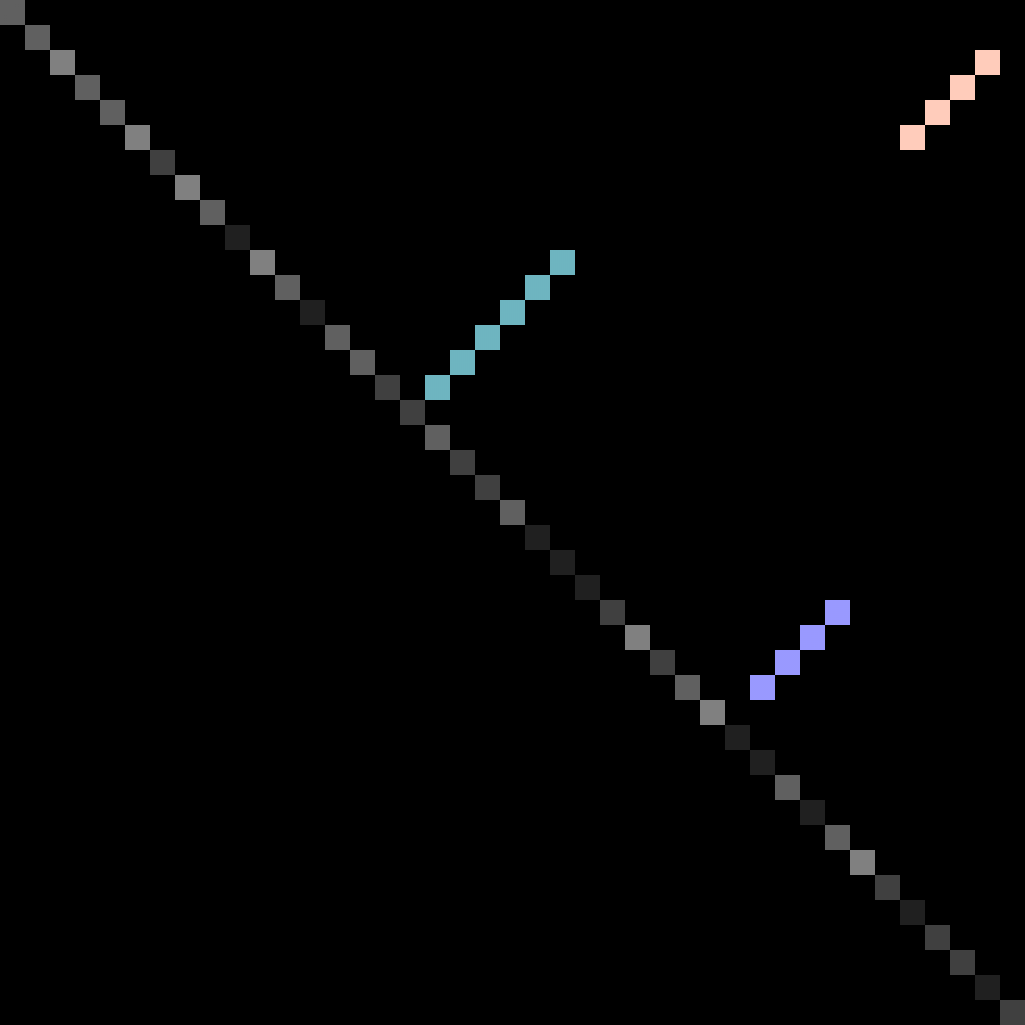
\includegraphics[width=.9\linewidth]{pics/out.png}}
  \caption{Эталонный  образец \\ для нейросети}
  \label{struc_b}
\end{subfigure}
\begin{subfigure}{.3\textwidth}
  \centering
  \fbox{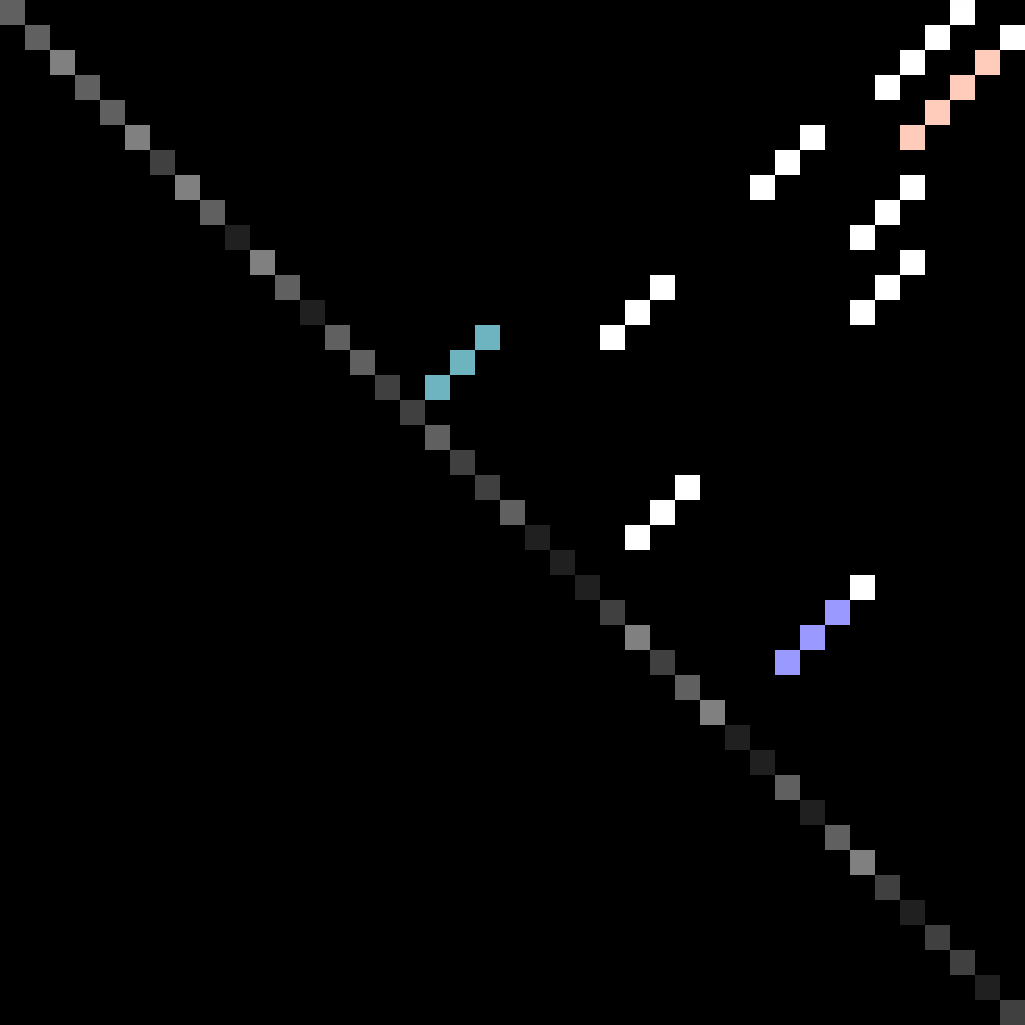
\includegraphics[width=.9\linewidth]{pics/in.png}}
  \caption{Входной образец \\ для нейросети}
  \label{struc_c}
\end{subfigure}
\caption{Примеры представления вторичной структуры}
\label{struc}
\end{figure}

Таким образом, в рамках данного исследования перед нейронной сетью стоит задача отфильтровать и дополнить матрицу разбора, сгенерировав корректную матрицу контактов, соответствующую максимально близкой к эталонной вторичной структуре.

\subsubsection{Параллельная остаточная архитектура}
Рассмотрим общую модель нейронной сети, разработанной в рамках данной работы. Входными и выходными данными являются изображения, и для решения поставленной задачи необходимо найти достаточно сложные закономерности между элементами данных, находящимися на большом расстоянии друг от друга, поэтому была использована глубокая сверточная сеть. Для оптимизации процесса обучения и повышения скорости сходимости была применена технология остаточных нейронных сетей. В процессе экспериментальных исследований нами было выявлено, что точность результатов значительно повышает использование $n$ остаточных сетей с одинаковой архитектурой, которые обучаются параллельно на одних и тех же данных, находя в них, по всей видимости, немного разные паттерны, а затем соединяются слоем, подсчитывающим линейную комбинацию их $n$ выходов и передающим ее уже общему остаточному блоку, завершающему обработку данных. Такая новая параллельная архитектура представлена на рис.~\ref{nn}; там же показано, как выглядит типичный остаточный блок (residual unit) нейронной сети, состоящий из пяти сверточных слоев с постепенно убывающими количеством фильтров и размером ядра свертки. В данной работе была использована модель, состоящая из четырех остаточных сетей с пятью одинаковыми блоками в каждой.

\begin{figure}[h]
\begin{center}
\centering
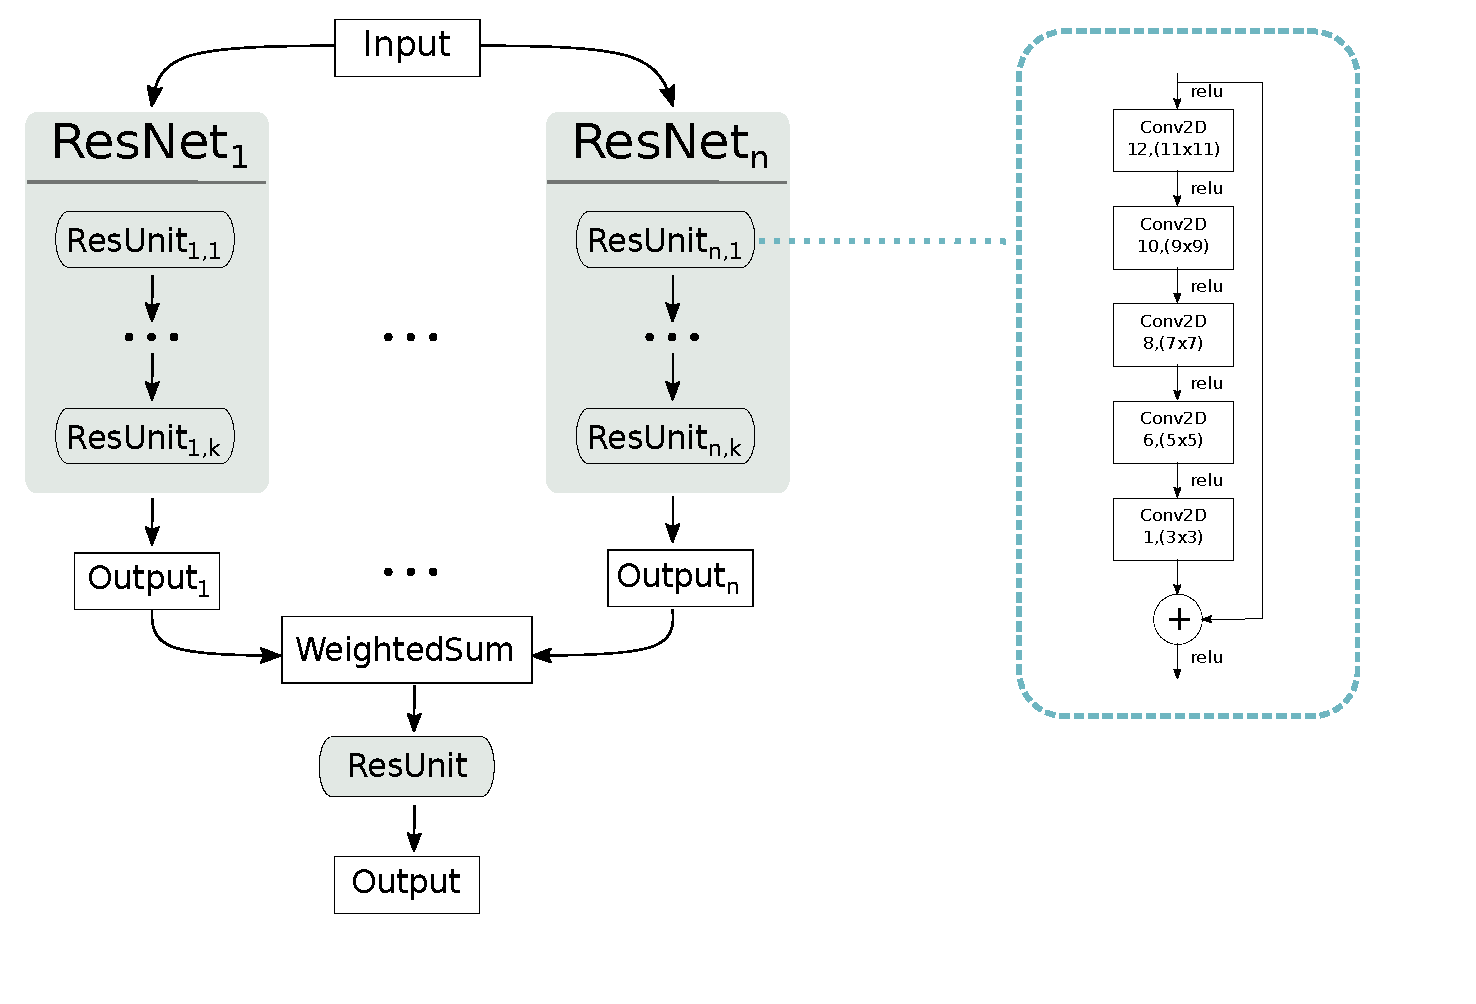
\includegraphics[width=15cm]{pics/nn.pdf}
\caption{Параллельная остаточная нейронная сеть}
\label{nn}
\end{center}
\end{figure} 